% EMNLP header. Do not change.
\pdfoutput=1
\documentclass[11pt]{article}
\usepackage[review]{emnlp2021}
\usepackage{times}
\usepackage{latexsym}
\usepackage[T1]{fontenc}
\usepackage[utf8]{inputenc}
\usepackage{microtype}
% End header.

%%%%%%%%%%%%%%%%%%%%
%%%%%%%%%%%%%%%%%%%%
% EDITING LINK: 
% https://www.overleaf.com/3575751412sjsdmszkxsyh
%%%%%%%%%%%%%%%%%%%%
%%%%%%%%%%%%%%%%%%%%

\usepackage{soul}
\usepackage{url}
% \usepackage[hidelinks]{hyperref}https://www.overleaf.com/project/614b5cc61d38655dce466002
% \usepackage[small]{caption}
\usepackage{graphicx}
\usepackage{amsmath}
\usepackage{amsthm}
\usepackage{booktabs}
\usepackage{algorithm}
\usepackage{algorithmic}
\urlstyle{same}

% =======================================
% my imported packages

\usepackage{amsmath}
\usepackage{bm}
\usepackage{amssymb}
\usepackage{listings}
% \usepackage[ruled,vlined]{algorithm2e}
\include{pythonlisting}

\newcommand{\pseudosection}[1]{\vspace{1.5ex}\noindent \textit{{#1:~~}}}
% \newcommand{\pseudosection}[1]\indent{{{}}}

\usepackage{todonotes}
\newcommand{\todokdinline}[1]{\todo[color=red!20,inline]{{KD: \small #1}}}
\newcommand{\todokd}[1]{\todo[color=red!20]{{\small #1 -- Kasra}}}
\newcommand{\todocainline}[1]{\todo[color=yellow!20,inline]{{CA: \small #1}}}
\newcommand{\todocm}[1]{\todo[color=green!40]{\small #1 -- Cynthia}}
\newcommand{\todocmi}[1]{\todo[inline,color=green!40]{\small #1 -- Cynthia}}
\newcommand{\todoff}[1]{\todo[color=blue!20]{\small #1 -- Frank}}
\newcommand{\todoed}[1]{\todo[color=cyan!20]{\small #1 -- Ed}}

\newcommand{\CitationNeeded}[1]{{\textbf {\color{red}Cite #1}}}
\newcommand{\ProofRead}[1]{{\textbf {\color{red}Proofread please #1}}}
\newcommand{\Complete}[0]{{\textbf {\color{red}Complete it }}}
\newcommand{\Rephrase}[1]{{\textbf {\color{red}Rephrase please #1}}}

% \newcommand{\citet}[1]{\cite{#1}} % This is used because \citet didn't work with their author kit % It does now

% =======================================

\title{MMA: Multi-modal Manifold Alignment \\ MAME: Manifold Alignment of Multimodal Embeddings}

\author{
First Author$^1$
\and
Second Author$^2$\and
Third Author$^{2,3}$\And
Fourth Author$^4$
\affiliations
$^1$First Affiliation\\
$^2$Second Affiliation\\
$^3$Third Affiliation\\
$^4$Fourth Affiliation
\emails
\{first, second\}@example.com,
third@other.example.com,
fourth@example.com
}


\begin{document}

Todo list

\begin{enumerate}
    \item \st{Lit search}
\end{enumerate}

\newpage

\maketitle
\setcounter{page}{1}

% ***************** The BEGINNING of the paper *****************

\begin{abstract}
    To be written ...
\end{abstract}

%===================================================================



\section{Introduction}
\label{intro}
Humans use multiple sensory inputs to interact with the world around them.
Most methods in machine learning use at most two sensory inputs that are very different such as visual data (such as RGB images) and natural language.
However, using extra similar inputs from different modalities is underexplored. This includes incorporating depth and RGB, written natural language and speech, and a combination of all of them.
Most of the proposed works cannot be extended to arbitrary number of modalities, and we address this shortcomings by proposing a generalized distance-based loss function.

% Grounded language learning~\cite{Mooney2008Grounded,RichardsDarvishMatuszekCategoryFree20,triplet_loss_2021_CVPR} is a cross-modal learning task to connect natural language with the physical environment in which the natural language is used.

\todokdinline{Are we doing contrastive learning? If so, mention it here}

Our contributions are as follows:
\begin{enumerate}
    \item Proposing a general distance-based loss function formulation for multimodal learning that can be extended to arbitrary number of modalities
    \item Outperforming state-of-the-art models for grounded language learning by treating depth image as its own separate channel.
    \item 
\end{enumerate}
%===================================================================


\section{Related Work}
\label{sec:Related-Work}
The growing number of multimodal datasets demonstrates the importance and the challenge of this task. \citet{bagher-zadeh-etal-2018-multimodal} introduce a large dataset of multimodal opinion sentiment and emotion intensity (CMU-MOSEI) for sentiment analysis and emotion recognition. They also introduce a novel multimodal fusion technique called the Dynamic Fusion Graph (DFG).
\citet{GoLD_UMBC} present a multimodal dataset of household objects containing RGB images, depth images, written language, and spoken language.

\citet{baltrusaitisMultimodalMachineLearning2019} propose a new taxonomy of multimodal machine learning by introducing five technical challenges in addition to typical early and late fusion categorization. They cover different approaches to multimodal machine learning such as \textit{representation}, \textit{translation}, \textit{alignment}, \textit{fusion}, and \textit{co-learning}. In this project, we focus on alignment.


We review different methods that have been proposed for alignment learning.
\citet{alayrac2020self} use a self-supervised contrastive learning method to learn and combine representations from three modalities of visual, audio, and language. Audio and visual domains are mapped to the same space because they are fine-grained, containing dense information for each frame of video. These embeddings are then mapped to a coarse space where text is also mapped. Their network respects specificity and comparability of different modalities. The loss function they define consists of two distance-based terms for the corresponding spaces. 

\citet{Nguyen-RSS-20} take a similar approach and perform pairwise cosine similarity to align images and natural language text descriptions to perform object retrieval.

\citet{triplet_loss_2021_CVPR} take a cross-modal manifold alignment approach to grounded language learning using triplet loss. They perform object retrieval by connecting text descriptions of objects to their corresponding RGB-D images.

Another related approach is contrastive learning which is based on the idea of similarity and distance~\cite{NEURIPS2020_supervised_contrastive,chen2020simple}. Triplet loss is also a special case of contrastive loss~\cite{NEURIPS2020_supervised_contrastive}.
Contrastive loss is mostly used in self-supervised learning~\cite{alayrac2020self,chen2020simple} with the exception of the work proposed by \citet{NEURIPS2020_supervised_contrastive} where they use contrastive loss for a supervised problem. Most of these methods are implemented for a unimodal dataset (i.e. dataset of one type of data such as RGB images only).



Some of the related works take more than two input modalities.
\citet{Veit_2018_CVPR} train a joint model of images, hashtags, and users to perform image retrieval. Their task is similar to our task where given a description, we want to find the image/object in the scene that best matches the description. Their idea to tackle this problem is to form a three-way tensor product model. They use a ranking loss to train the model where the score of an observed triplet is higher than an unobserved triplet. They sample six negative triplets per positive sample triplet, and use each of them as a negative in the loss.
The downstream retrieval task is then simply done by taking the arg max of the tensor product for a given user.


\citet{semihet_three_way_Lei_2020} use inputs from three modalities of image, sketch, and edgemap to perform image retrieval given the sketch. They use co-attention mechanism, and their loss function contains alignment loss, cross-entropy loss, and sketch-edgemap contrastive loss.
\citet{Mittal2020M3ER} use Canonical Correlational Analysis (CCA) to differentiate between ineffective and effective modalities for the emotion recognition task from multiple input modalities including face, speech, and text.

Multimodal learning has been used for different applications including but not limited to object retrieval. \citet{Deception_ICMI_2014} use \textit{language}, \textit{physiological response}, and \textit{thermal sensing} to detect deceit. \citet{het_data_fusion_liu_IEEE_2017} take two modalities as input and output predictions in a third modality.




\todo[inline]{talk about CLIP and DALL-E here}

However, to the best of our knowledge, there has not been any work to incorporate more than 3 modalities, and that's the novelty of our work.





%===================================================================

\section{Problem Description}
\label{sec:Problem-Description}











%===================================================================



\section{Approach}
\label{sec:Method}

For $M$ modalities, we define a distance based loss function that contains $M+2(M-1)!$ terms. 
We sample two data points from each modality, one positive point and one negative point. The objective is then to (I) minimize the distance between each pair of positive points from heterogeneous modalities which results in $(M-1)!$ terms, (II) maximize the distance between each pair of positive and negative points from heterogeneous modalities which contains $(M-1)!$ terms again, and (III) maximize the distance between each pair of positive and negative points from the homogeneous modalities which contains $M$ terms.
Equation~\ref{eq:objective} shows the objective function we defined above with changing maximization to minimization by changing the sign.

% \begin{equation}\label{eq:objective-detailed}
%     \min \sum_{i=1}^{M-1} \sum_{j=i+1}^{M} ||x_{i}^{+} - x_{j}^{+}|| - \sum_{i=1}^{M-1} \sum_{j=i+1}^{N} ||x_{i}^{+} - x_{j}^{-}|| - 
%     \sum_{i=1}^{M} ||x_{i}^{+} - x_{i}^{-}||
% \end{equation}


\begin{equation}\label{eq:objective}
\begin{split}
    \mathcal{L}  &= \sum_{i=1}^{M-1} \sum_{j=i+1}^{M} ||f_i(x_{i}^{+}) - f_j(x_{j}^{+})|| \\
    & - ||f_i(x_{i}^{+}) - f_j(x_{j}^{-})||
    - ||f_i(x_{i}^{-}) - f_j(x_{j}^{+})|| \\
    & - \sum_{i=1}^{M} ||f_i(x_{i}^{+}) - f_i(x_{i}^{-}) ||
\end{split}
\end{equation}
where the subscripts $i$ and $j$ represent modalities, and $f_i(.)$ and $f_j(.)$ represent functions that map input data to the shared latent space using a deep neural network.

\todokdinline{I can add another term for minimizing the distance between similar pairs (anchor and positive) from the same domain. This would look like the equation below. However, it breaks the nice procedure of sampling two data points per modality}
$+ \sum_{i=1}^{M} ||f_i(x_i^{a}) - f_i(x_i^{+})||$

Our method is a generalization of well-known similarity-based metric learning and manifold alignment methods such as triplet loss~\cite{Carvalho-cooking-triplet,triplet_loss_2021_CVPR}.
If $M=2$ which means the number of modalities is 2, then our objective function reduces to quadruplet loss method.
If $M=2$ and we ignore the last term in the objective function, it results in the triplet loss method. 
If $M=1$, only the last term remains in the loss function which is exactly the pairwise distance-based loss function.


\subsection{Loss Functions}
We try three different distance based loss functions.
In order to use cosine distance, we have to subtract the cosine between two embeddings from 1 which means $1 - \cos(e_1, e_2)$.

\subsubsection{Simple triplet extension}
\label{sub:simple-mma}

First one is a modification of the triplet loss function idea. For each data point (referring to an instance of an object with all of its modalities), we choose a negative data point either based on object class name, or by negative sampling~\cite{Pillai_Matuszek_2018}. We now have two data points; we consider the first one as positive, and the second one as negative. However, the anchor won't be another data point as it is in the triplet loss terminology. Instead we choose one domain as an anchor. 

\begin{itemize}
    \item data point: a row in the csv/tsv file.
    \item Positive: a set of embeddings of the one data point (rgb image of an apple, depth image of an apple, language description of an apple)
    \item Negative: a set of embeddings of the another data point of a different object (rgb image of a book, depth image of a book, language description of a book)
    \item Anchor: A fixed modality to act as anchor in the case of simple MMA loss, where we don't minimize the distance between the pair of embeddings from all modalities of the same data point, and we don't maximize the distance between positive an negative datapoints of the same modality.
\end{itemize}

Since the downstream task is to predict/retrieve the desired object among multiple objects given a natural language description, it makes sense to train the model using language as anchor. 
We tried RGB as anchor, and as expected the performance was worse.

Equation~\ref{eq:objective-simple-mma} shows the mathematical formulation of the proposed loss function which can be generalized to arbitrary number of modalities.

\begin{equation}
\label{eq:objective-simple-mma}
\begin{split}
    \mathcal{L}  &= \sum_{m=1}^{M-1} || f_a(x_{a}^{+}) - f_m(x_{m}^{+}) || - \\ 
    & || f_a(x_{a}^{+}) -f_m(x_{m}^{-}) || 
    \\
    &= \sum_{m=1}^{M-1} 1 - \cos(f_a(x_{a}^{+}), f_m(x_{m}^{+})) \\ & - (1 - \cos(f_a(x_{a}^{+}) ,f_m(x_{m}^{-}))) \\
    &= \sum_{m=1}^{M-1} \cos(f_a(x_{a}^{+}) ,f_m(x_{m}^{-})) \\ 
    & - \cos(f_a(x_{a}^{+}), f_m(x_{m}^{+}))
\end{split}
\end{equation}

where $a$ represents \textit{anchor} modality, $M$ is the number of modalities, $p$ represents the positive objects, and $n$ represents the negative objects.

An illustration of this loss function is provided in figure~\ref{fig:simple-mma-loss}.

This version of MMA loss function can be seen as a contrastive loss usually used in the domain of self-supervised learning~\cite{chen2020simple}. However, our proposed loss function has two advantages over the traditional contrastive loss expressed in equation~\ref{eq:contrastive-loss}. The first advantage is that our loss function do not loop over multiple positives and negatives in a large batch. Instead we sample only two objects (positive and negative) each of which have $M$ modalities which gives us $2M$ datapoints (or embeddings). Hence, our model can be trained using smaller batch sizes and reduces the number of negative samples we need. Second advantage is that this loss function can be used in a multimodal setting with an arbitrary number of modalities, and is not limited to a single data type (e.g. RGB images) which is the most common usage of contrastive loss~\cite{chen2020simple, NEURIPS2020_supervised_contrastive}.

\begin{equation}\label{eq:contrastive-loss}
    -\sum_{i \in I} \log \frac{\exp (z_i . z_{j(i)} / \tau) }{\sum_{a \in A(i)} \exp (z_i.z_a / \tau)}
\end{equation}


Therefore, our proposed loss function would modify the equation~\ref{eq:contrastive-loss} to the loss function formulated in equation~\ref{eq:simple-MMA-contrastive}. Our formulation is a generalized version of the contrastive loss where $M$ is the number of modalities (e.g. RGB image, depth image, speech, text), but it can be the ``augmented views'' instead of different modalities.

\begin{equation}\label{eq:simple-MMA-contrastive}
    -\sum_{m=1}^{M-1} \log \frac{\exp (z_a . z_{m}^{+}/ \tau) }{ \exp (z_a.z_m^{+} / \tau) + \exp (z_a.z_m^{-} / \tau)}
\end{equation}

\todokdinline{I should run the traditional contrastive loss to see if my method works better to make this claim.}





\begin{figure*}[tbh]
\centering
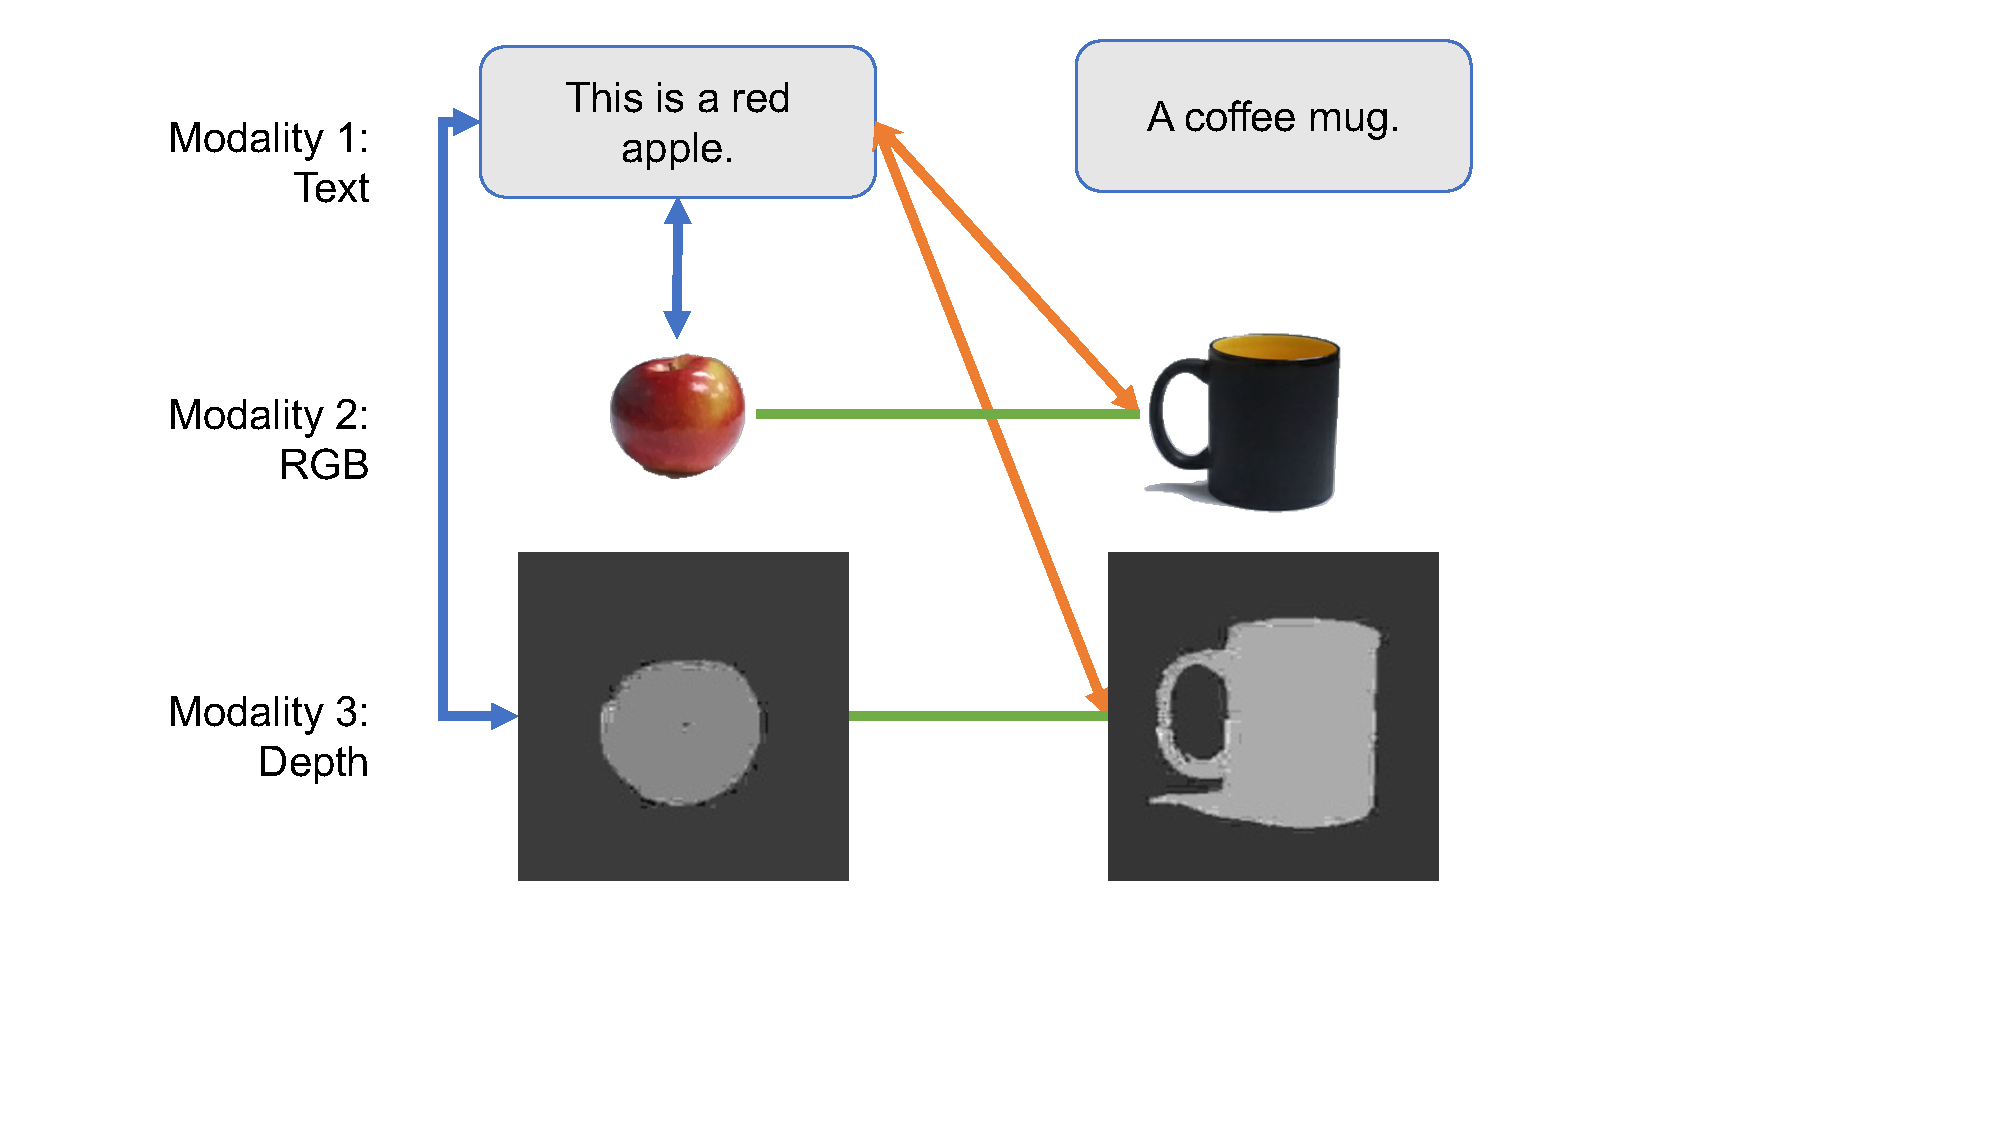
\includegraphics[width=2.0\columnwidth]{Figures/simple-MMA.pdf}
\caption{A high-level prototype of the distances used in the simple MMA loss with 3 modalities. Orange arrows indicate maximizing the distance, blue arrows indicate minimizing the distance, and green arrows show the margin.}
\label{fig:simple-mma-loss}
\end{figure*}





\subsubsection{All in loss with 12 terms}
\subsubsection{subset of All in loss with 9 terms}






\subsection{Network Architecture}
\label{sec:Model}

We use BERT \CitationNeeded{} to featurize the textual input, and wave2vec2 \CitationNeeded{} to extract audio embeddings from speech both of which output a 3072-dimensional embedding vector.
To process images, we use ResNet152 \CitationNeeded{} for both RGB and depth images which gives us a 2048-dimensional embedding vector.
We then use 3 fully connected layers to map these embeddings to a shared 1024-dimensional space where we can compute the distance between all embeddings.







%===================================================================


\section{Experiments}
\label{sec:Experiments}

\subsection{4 Modalities}
We ran an experiment with RGB, depth, language. The loss function doesn't require any changes beyond increasing the number of loops in equation~\ref{eq:objective-simple-mma} (or increasing the value of $M$ by 1).
The non-trivial part is the downstream prediction task. In the case of three modalities, language is the anchor, and we compute the distance of other two modalities from it and then average them.
With speech coming into the picture, we have three choices.
First, treat it in a similar way to RGB and depth; which means computing the distance of RGB, depth, and speech from text, and then take an average of three of them.
Second way is to compute the distance of RGB and depth from language and from speech which gives us 4 distance matrices, and then take average of the 4 of them.
Third way is similar to the second methods, but we compute the distance between language and speech as well and then take average of 5 distance matrices.
The problem with second and third method, is that the simple MMA loss function in equation~\ref{eq:objective-simple-mma} is not designed in a way to minimize the distance between speech and visual embeddings explicitly. This is supported by our experimental results where the first method results in a better performance compared to the other two methods.
Third method (averaging 5 matrices) is the worst, then second one (averaging 4 matrices) is bad. First method has the best results.

\todokdinline{try the more complicated MMA that might be able to capture these relationships.}


\subsection{Contrastive Loss}
We compare our model against contrastive loss as formulated in equation~\ref{eq:contrastive-loss}.
In order to implement this loss function, we use cosine similarity as suggested in the SimCLR paper~\cite{chen2020simple}.
The other version mentioned by~\citet{NEURIPS2020_supervised_contrastive} uses inner dot product which can lead to instabilities since the dot product is not bounded.
\todokdinline{try contrastive loss with cross-entropy, dot product, and the supervised contrastive method itself (without triplets).}


\subsection{Metrics}
\label{sec:metrics}
To evaluate our model we measure different performance metrics on a retrieval task where the model has to select 1 object among 5 objects given a language description. Only one of the objects corresponds to the description and the rest are from different object classes.
\todokdinline{Try with different number of objects.}


To evaluate the performance, we compute the cosine distance between a given natural language description and 5 randomly selected images (1 of which corresponds to the description, and others are from different object classes). We have to modify the way we compute the distance since we treat depth images as a separate input modality and do not append it to the RGB features as in the triplet loss method~\cite{triplet_loss_2021_CVPR}.
To handle this, we compute the distance between 1 language embedding and all candidate RGB embeddings, and we compute the distance between the same language embedding and all candidate depth embeddings corresponding to the RGB embeddings. We then take average of these two distance matrices.

Moreover, instead of choosing an arbitrary threshold, we choose the closest image embedding (average distance of rgb and depth from language) as the prediction.

The best metric to capture the performance in such a scenario would be mean reciprocal rank (MRR) and accuracy.
Accuracy, micro F1 score (sklearn), flatten binary f1 score (sklearn), and my f1 score computation are all the same in this task since for each prediction we either have a true positive and no false positives and no false negatives (no FP no FN), or we have no true positives and 1 false positive and 1 false negative.
However, subset MRR is equal or greater than those because if the model do not rank the correct answer as 1, it still gets some score and is greater than 0 (in accuracy the score is ether 0 or 1).

\subsection{Data}
\label{sec:Data}

We use a recent multimodal dataset called GoLD~\cite{GoLD_UMBC}. The original paper uses raw RGB and raw depth images in which other items are present in the background. We use a masked version of the images where the background (including the white turntable) is deleted and one object is present in each image.
We show that a masked version converges faster, however, they both converge to the same performance after enough epoch as shown  in figure~\ref{fig:mask-vs-raw}.

\begin{figure*}[tbh]
\centering
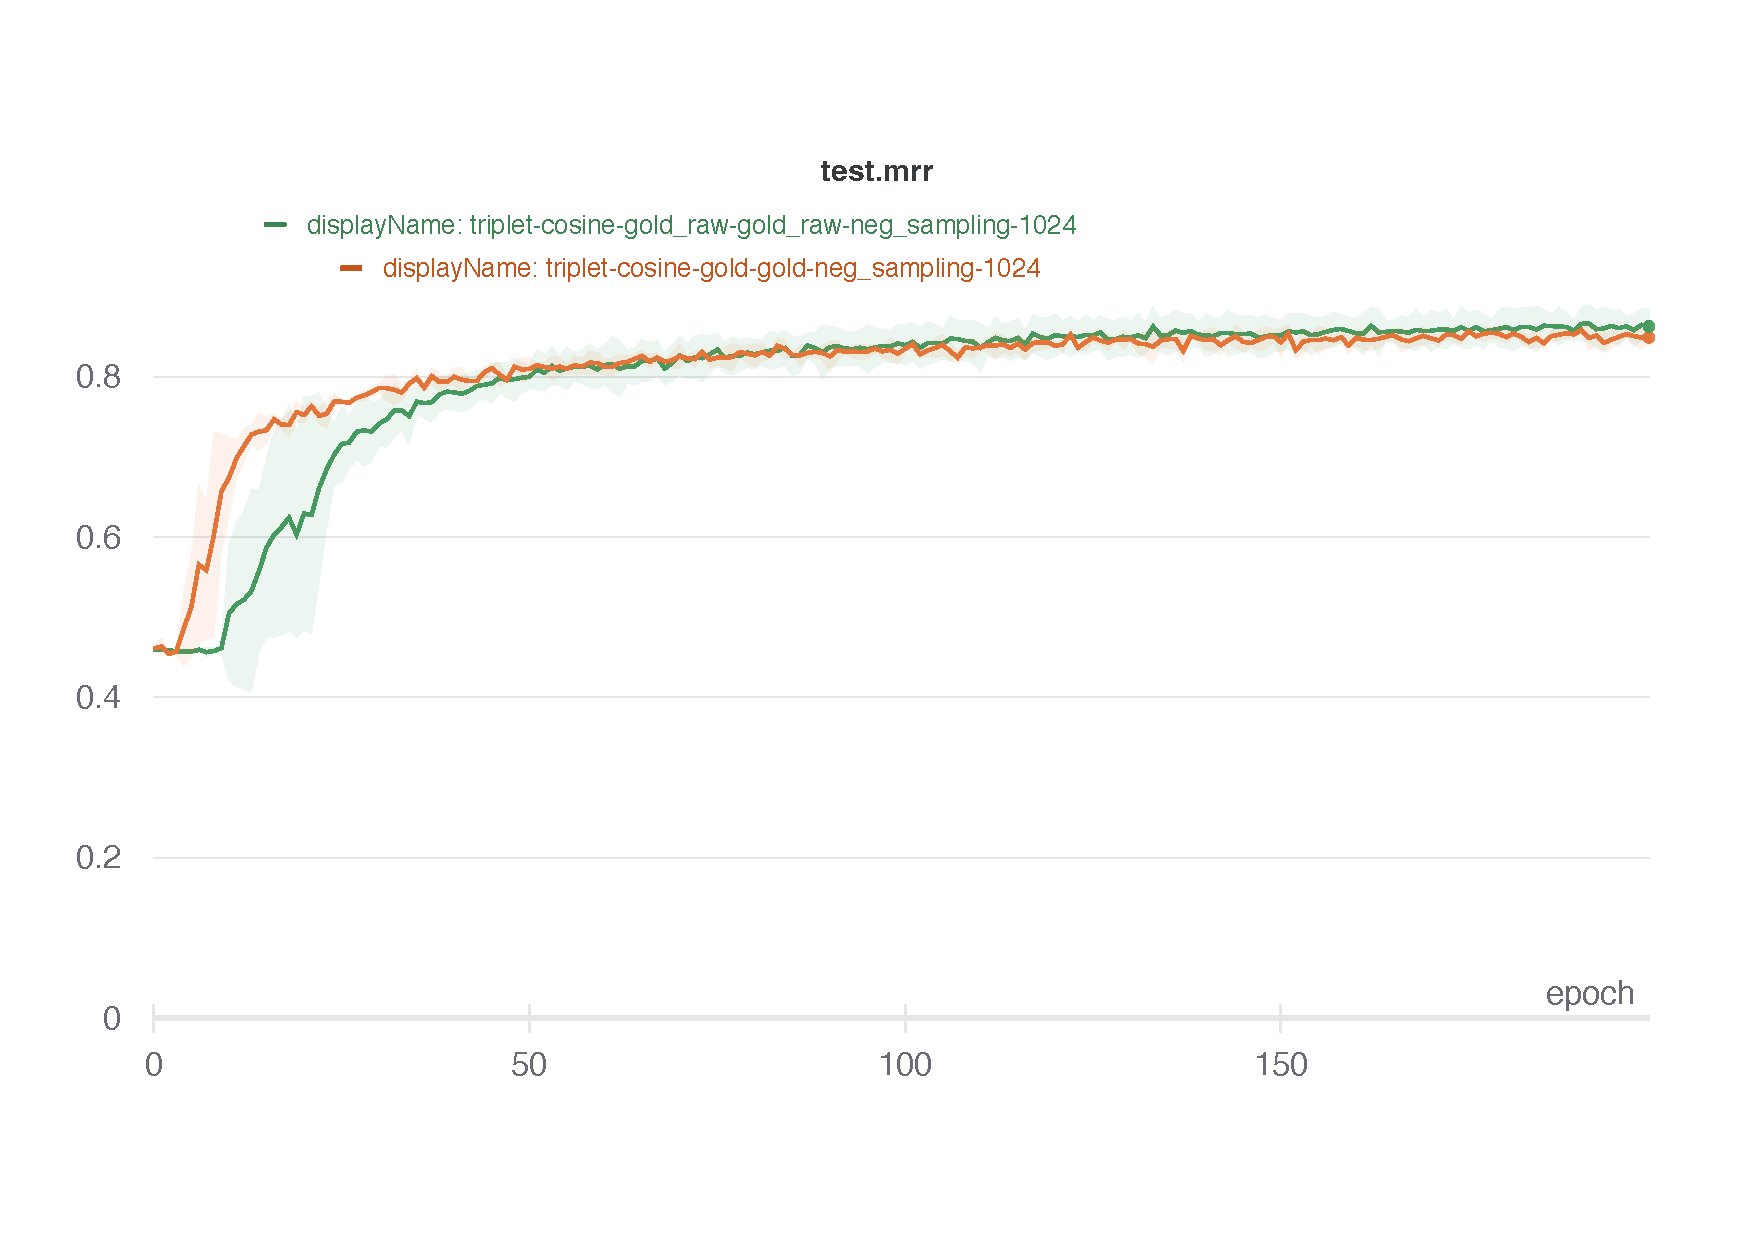
\includegraphics[width=2.0\columnwidth]{Figures/raw-mask-test-mrr.pdf}
\caption{Mean Reciprocal Rank (MRR) on different versions of GoLD dataset~\cite{GoLD_UMBC}. The raw version is depicted in green and masked version is depicted in orange averaged over 3 different random seeds. The higher is better.}
\label{fig:mask-vs-raw}
\end{figure*}


Since the wave2vec2~\CitationNeeded{} model is trained on 16hz speech data, we need to convert he speech files to 16hz.



\subsection{Setup}
\label{sec:setup}

We use \Complete optimizer with a learning rate of \Complete.
The models are trained for \Complete epochs on a \Complete GPU.




\subsection{Baselines}
We compare our MMA model against the triplet loss method proposed by~\citet{GoLD_UMBC} and~\citet{triplet_loss_2021_CVPR}. Triplet loss function consists of three data points including anchor, positive, and negative from two modalities. The anchor, positive, and negative can be chosen from different modalities in each batch.
The triplet loss method has two major disadvantages. First, it cannot be used for more than three modalities since there are only 3 data points in the loss function. Second, a batch size of greater than 1 cannot be easily implemented if the anchor, positive, and negative come from different modalities for each batch.
To address this issues, we sample more than one positive and one negative data points. Essentially, we sample one positive data point and one negative data point from each modality which results in 2(M-1) + 1 data points where 1 is the single anchor data point from anchor modality of the same object class as positive datapoints. We would have 2M datapoints if we use the negative data point from the anchor modality too. The anchor data point is always from the same modality and corresponds to the same object class sampled for positive data points.

\subsection{Quantitative Results}
\label{sec:Quantitative}

We evaluate our proposed simple MMA loss function~\ref{sub:simple-mma} against the triplet loss method~\cite{triplet_loss_2021_CVPR}. Our model significantly outperforms the triplet method across all epochs while it converges faster as shown in figure~\ref{fig:simple-MMA-mrr}.
Table~\ref{table:quantitative} summarizes the performance of all models.

\begin{table*}[tbh]
\centering
\begin{tabular}{|c|c|c|}
\toprule
\textbf{Method} & \textbf{Accuracy} & \textbf{MRR} \\ %\hline
\midrule
Full MMA (Text) w/ neg & ?$\pm$? & ?$\pm$? \\
Simple MMA (Text) w/ neg & \textbf{0.7949}$\pm$? & \textbf{0.8778}$\pm$? \\
Contrastive (Text) w/ neg & ?$\pm$? & ?$\pm$? \\
Triplet (Text) w/ neg & 0.7497$\pm$? & 0.8522$\pm$? \\
Full MMA (Speech) w/ neg & ?$\pm$? & ?$\pm$? \\
Simple MMA (Speech) w/ neg & \textbf{0.7949}$\pm$? & \textbf{0.8778}$\pm$? \\
Contrastive (Speech) w/ neg & ?$\pm$? & ?$\pm$? \\
Triplet (Speech) w/ neg & 0.7497$\pm$? & 0.8522$\pm$? \\
Triplet (Speech) w/o neg & 0.7497$\pm$? & 0.8522$\pm$? \\
\bottomrule
\end{tabular}
\caption{\label{table:quantitative}Average and standard deviation of accuracy and MRR over 3 runs with 3 different random seeds on a hel-out test set. Both metrics are from 0 to 1, and the higher is better.\todokdinline{maybe adding results on cropped and raw dataset as well. Also results using objec class isntead of negative sampling}}
\end{table*}


\begin{figure*}[tbh]
\centering
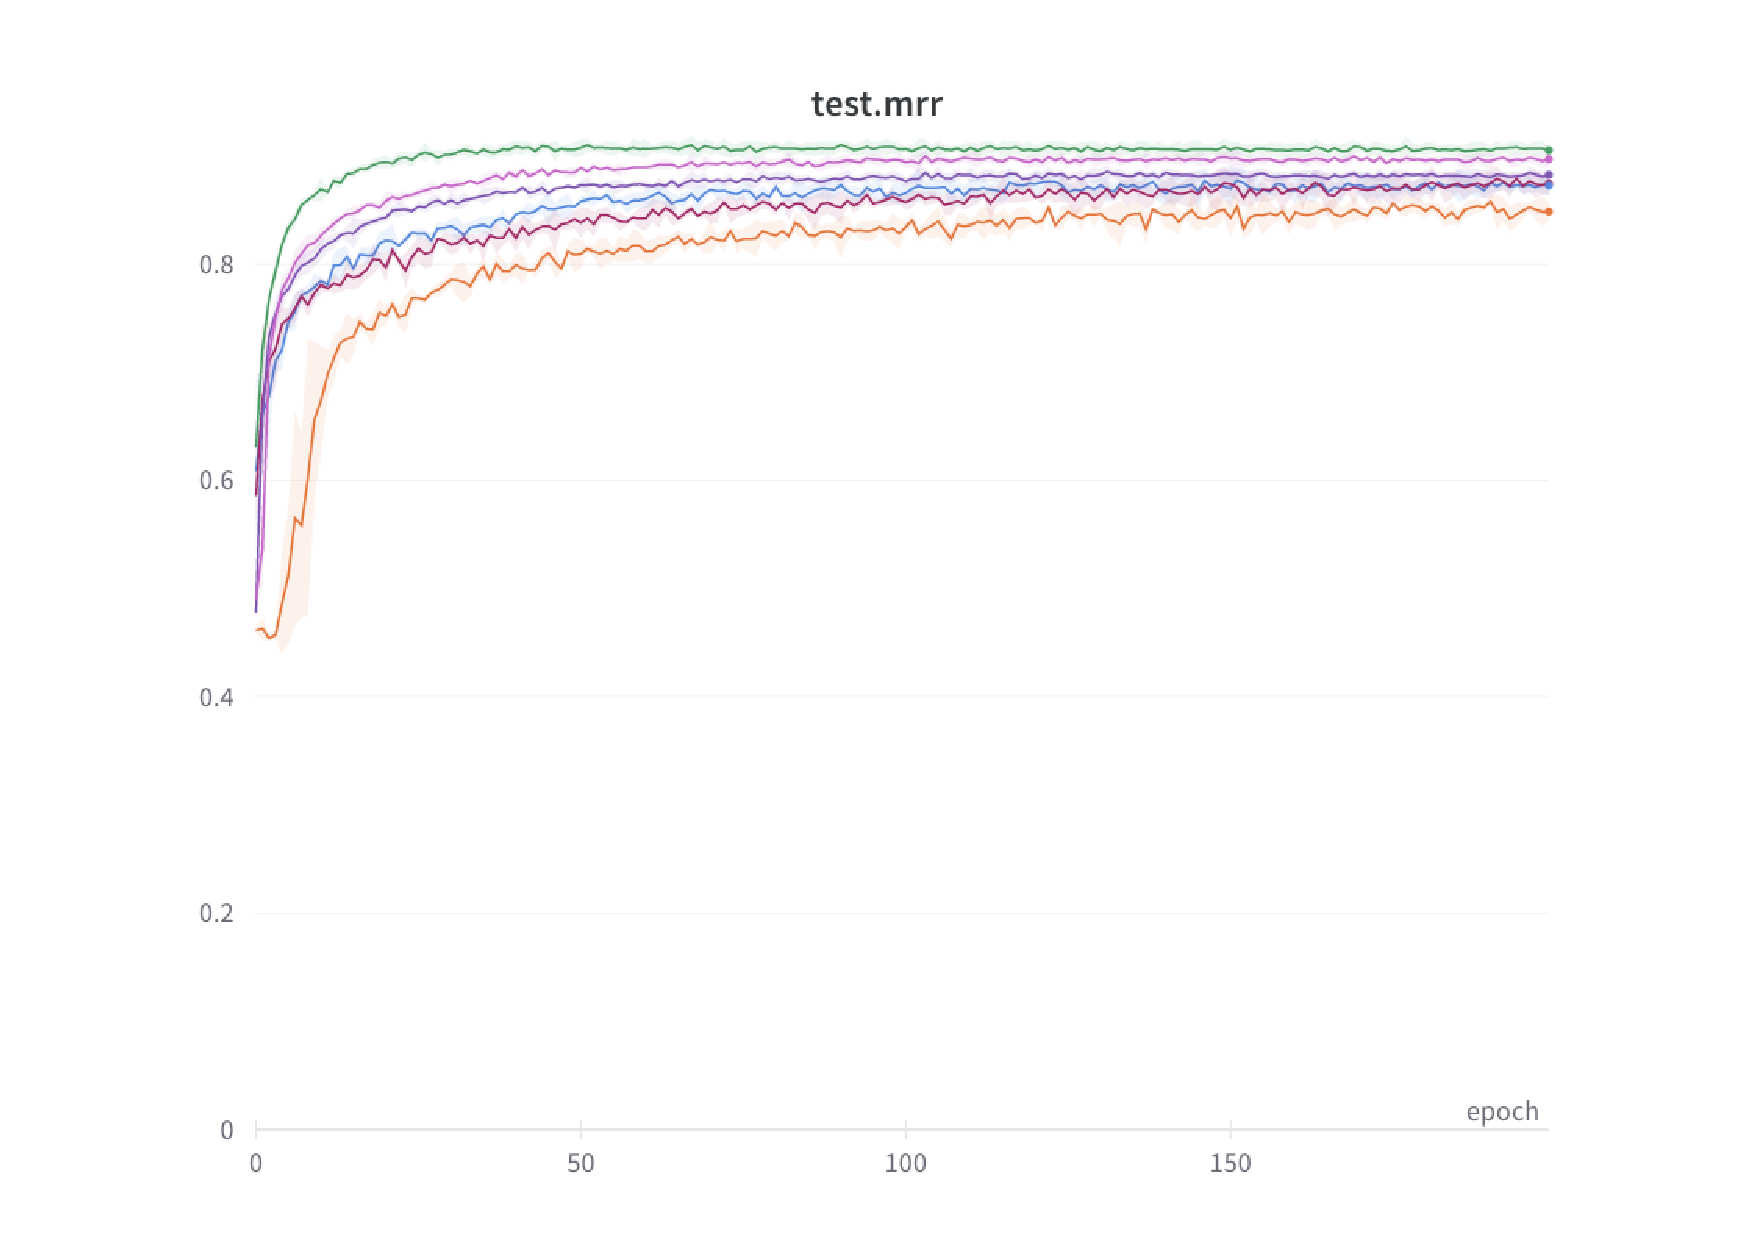
\includegraphics[width=2.0\columnwidth]{Figures/test.mrr.pdf}
\caption{Mean Reciprocal Rank (MRR) of our proposed method against triplet loss method averaged over 3 different random seeds for a downstream task of object detection. The higher is better. Blue represents our proposed simple MMA loss function, and orange represent the triplet loss function~\cite{triplet_loss_2021_CVPR}.}
\label{fig:simple-MMA-mrr}
\end{figure*}


\subsection{Qualitative Results}
\label{sec:Qualitative}












%===================================================================





\section{Conclusion}
\label{sec:conclusion}


%===================================================================


% ***************** The END of the paper *****************


\clearpage
\clearpage
\section*{Acknowledgments}
%% The file named.bst is a bibliography style file for BibTeX 0.99c
\bibliographystyle{named}
\bibliography{ref}
\clearpage

\appendix
\label{sec:appendix}


\section{Qualitative Analysis}

\section{Model}


\section{Experiments}

\section{Results}

\section{Setup}

\section{Lit Search}
\subsection{Multimodal Machine Learning: A Survey and Taxonomy}

\begin{itemize}
\item \href{https://ieeexplore.ieee.org/document/8269806}{url}
\end{itemize}

\citet{baltrusaitisMultimodalMachineLearning2019} proposes a new taxonomy of multimodal machine learning by introducing five technical challenges in addition to typical early and late fusion categorization. This taxonomy includes the following categories.
\begin{enumerate}
\item \textit{Representation}: represent and summarize multimodal data in a way that exploits the complementarity and redundancy of multiple modalities.
\begin{enumerate}
\item joint: combine the unimodal signals into the same representation space.
\item coordinated: process unimodal signals separately, but enforce certain similarity or structure constraints on them to bring them to a coordinated space.
\end{enumerate}
\item \textit{Translation}: map data from one modality to another.
\begin{enumerate}
\item example-based
\item generative
\end{enumerate}
\item \textit{Alignment}: identify the direct relations between (sub)elements from two or more different modalities.
\begin{enumerate}
\item explicit
\item implicit
\end{enumerate}
\item \textit{Fusion}: join information from two or more modalities to perform a prediction.
\begin{enumerate}
\item model-agnostic
\item model-based
\end{enumerate}
\item \textit{Co-learning}: transfer knowledge between modalities, their representation, and their predictive models
\begin{enumerate}
\item parallel data
\item non-parallel data
\item hybrid data
\end{enumerate}
\end{enumerate}

The authors mention that while joint representations have been used in situations to construct representations of more than two modalities, coordinated spaces have, so far, been mostly limited to two. This means that our research is novel and we can extend similarity measures to more than two modalities.

\subsection{Self-Supervised MultiModal Versatile Networks}

\begin{itemize}
\item \href{https://proceedings.neurips.cc/paper/2020/file/0060ef47b12160b9198302ebdb144dcf-Paper.pdf?utm\_campaign=NLP\%20News\&utm\_medium=email\&utm\_source=Revue\%20newsletter}{url}
\end{itemize}


This work uses self-supervised contrastive learning to learn and combine representations from three modalities of visual, audio, and language. They learn a \textit{multimodal versatile network} that has the following four properties:
\begin{enumerate}
\item Ability to take any of the modalities as input
\item Respecting the specificity of modalities: audio and visual modalities are fine-grained while language modality is coarse-grained.
\item Comparability of different modalities using \textbf{dot product} even if not seen together during training 
\item Efficiently applicable to visual data either in the form of dynamic videos or static images
\end{enumerate}


The authors consider the following three different configurations of the modality spaces which they call \textit{modality embedding graphs}.
\begin{enumerate}
\item Shared: all modalities map to the same space. This respects property 3 but violates property 2.
\item Disjoint: visual-audio and visual-text spaces. This respects property 2 but violates property 3.
\item Fine and coarse: audio and visual domains are map to the same space since they are fine-grained. These embeddings are then mapped to a lower dimensional space where text is also mapped. This respects both properties 2 and 3.
\end{enumerate}

The loss function they define consists of two terms. The first term is to train the fine-grained space of visual and audio embeddings by minimizing the distance between the similar pair (positives) from the same location of a video, and maximizing the distance between negative pairs (negatives) sampled from different videos. The second term is to train the coarse-grained space which consists of visual and text embeddings. Note that they don't consider audio embeddings in this space since they don't want to learn automatic speech recognition (ASR). Text and visual domains are not aligned as well as audio and visual domains (e.g. sound of playing piano versus the text that only says playing piano for a video of playing piano). To cure this, they consider a set of positive pairs instead of a single pair.
If a modality is missed, the corresponding term is dropped from the loss function.

\subsection{Separating Self-Expression and Visual Content in Hashtag Supervision}

\begin{itemize}
\item \href{https://openaccess.thecvf.com/content\_cvpr\_2018/papers/Veit\_Separating\_Self-Expression\_and\_CVPR\_2018\_paper.pdf}{url}
\end{itemize}

The authors train a joint model of images, hashtags, and users to perform image retrieval. This is similar to our task where given a description, we want to find the image in the scene that best matches the description. The idea is to form a three-way tensor product model. They use a ranking loss to train the model where the score of an observed triplet is higher than an unobserved triplet. They sample six negative triplets per positive sample triplet, and use each of them as a negative in the loss.
The downstream retrieval task is then simply done by taking the arg max of the tensor product for a given user.



\subsection{Semi-Heterogeneous Three-Way Joint Embedding Network for Sketch-Based Image Retrieval}

\begin{itemize}
\item \href{https://ieeexplore.ieee.org/document/8809264}{url}
\end{itemize}

\subsection{Deep Multimodal Learning for Affective Analysis and Retrieval}

\begin{itemize}
\item \href{https://ieeexplore.ieee.org/abstract/document/7277066?casa\_token=aBp6BxcszHwAAAAA:3NoMiFrZbn7tXfavF1rgkCiGWbFI2arxn8Xb6iDF79q4zBZHWi7PWWhf6xW-xJwYdFALbmRENo4}{url}
\end{itemize}

\subsection{An Efficient Framework for Zero-Shot Sketch-Based Image Retrieval}

\begin{itemize}
\item \href{https://arxiv.org/pdf/2102.04016.pdf}{url}
\end{itemize}
This paper uses two modalities only; image and sketch. However, it uses a \textit{quadruplet} to compute the loss which can be useful in our research. A quadruplet is composed of a sketch picture as an anchor, a negative example from sketch domain, a negative example from picture domain, and a positive example from picture domain.

\subsection{SMIL: Multimodal Learning with Severely Missing Modality}

\begin{itemize}
\item \href{https://www.aaai.org/AAAI21Papers/AAAI-437.MaM.pdf}{url}
\end{itemize}
Uses Bayesian meta-learning framework to perform multimodal learning with partially missing modalities in training/test data.
One of their experiments is multi-label classification of movie genres with bimodal data including poster of movies and description of the movie from IMDB.

\subsection{Multimodal Language Analysis in the Wild: CMU-MOSEI Dataset and Interpretable Dynamic Fusion Graph}

\begin{itemize}
\item \href{https://aclanthology.org/P18-1208.pdf}{url}
\end{itemize}

\subsection{Multimodal Learning with Incomplete Modalities by Knowledge Distillation}

\begin{itemize}
\item \href{https://dl.acm.org/doi/pdf/10.1145/3394486.3403234}{url}
\end{itemize}
They first train models on each modality independently
\subsection{SWAFN: Sentimental Words Aware Fusion Network for Multimodal Sentiment Analysis}

\begin{itemize}
\item \href{https://aclanthology.org/2020.coling-main.93.pdf}{url}
\end{itemize}

\subsection{Multimodal Learning for Human Action Recognition Via Bimodal/Multimodal Hybrid Centroid Canonical Correlation Analysis}

\begin{itemize}
\item \href{https://ieeexplore.ieee.org/document/8489981}{url}
\end{itemize}

\subsection{Deception Detection Using a Multimodal Approach}

\begin{itemize}
\item \href{https://dl.acm.org/doi/pdf/10.1145/2663204.2663229?casa\_token=KneK7B7xvLwAAAAA:Ajz0N96ygq8ktwkz0IVUqTt8NozCg2wR6n\_x2xntdHqZBh6VXW\_8VbO4GeY4VvMsDJlMwzkhVXQSJA}{url}
\end{itemize}
They use \textit{language}, \textit{physiological response}, and \textit{thermal sensing} to detect deceit.

\subsection{M3ER: Multiplicative Multimodal Emotion Recognition using Facial, Textual, and Speech Cues}

\begin{itemize}
\item \href{https://ojs.aaai.org/index.php/AAAI/article/view/5492}{url}
\end{itemize}

\subsection{Found in Translation: Learning Robust Joint Representations by Cyclic Translations between Modalities}

\begin{itemize}
\item \href{https://ojs.aaai.org/index.php/AAAI/article/view/4666}{url}
\end{itemize}
\subsection{Select-Additive Learning: Improving Generalization In Multimodal Sentiment Analysis}

\begin{itemize}
\item \href{https://ieeexplore.ieee.org/stamp/stamp.jsp?tp=\&arnumber=8019301}{url}
\end{itemize}

\subsection{Attention-Based Multimodal Fusion for Video Description}

\begin{itemize}
\item \href{https://openaccess.thecvf.com/content\_ICCV\_2017/papers/Hori\_Attention-Based\_Multimodal\_Fusion\_ICCV\_2017\_paper.pdf}{url}
\end{itemize}
\subsection{\st{3W-AlignNet: a Feature Alignment Framework for Person Search with Three-Way Decision Theory}}

\begin{itemize}
\item \href{https://link.springer.com/article/10.1007/s12559-021-09898-7}{url}
\end{itemize}

This is not very related since they use three-way decision theory to select bounding boxes as positive, negative, and boundary.
Three-way here refers to something else and not modalities.

\subsection{\st{Unsupervised Domain Adaptation for Face Recognition in Unlabeled Videos}}
\begin{itemize}
\item \href{https://openaccess.thecvf.com/content\_ICCV\_2017/papers/Sohn\_Unsupervised\_Domain\_Adaptation\_ICCV\_2017\_paper.pdf}{url}
\end{itemize}
Might be relevant but not super relevant.


\subsection{Heterogeneous Sensor Data Fusion By Deep Multimodal Encoding}
\begin{itemize}
\item \href{https://ieeexplore.ieee.org/stamp/stamp.jsp?tp=&arnumber=7874158}{url}
\end{itemize}
This one takes two modalities as input and outputs predictions in a third modality.

\subsection{Multimodal Contrastive Training for Visual Representation Learning}
\href{https://arxiv.org/pdf/2104.12836.pdf}{paper pdf}


\subsection{CrossCLR: Cross-modal Contrastive Learning For Multi-modal Video Representations}
\href{https://openaccess.thecvf.com/content/ICCV2021/papers/Zolfaghari_CrossCLR_Cross-Modal_Contrastive_Learning_for_Multi-Modal_Video_Representations_ICCV_2021_paper.pdf}{paper pdf}

%===================================================================





\end{document}

